\documentclass[12pt,a4paper,titlepage]{article}
\usepackage[utf8]{inputenc}
\usepackage[finnish]{babel}
\usepackage{setspace}
\usepackage{parskip}
\usepackage{amssymb}
\usepackage{amsmath}
\usepackage{graphicx}
\usepackage{fancyhdr}
\usepackage[top=1in, bottom=1in, left=1in, right=1in]{geometry}
\usepackage{float}
\usepackage[section]{placeins}
\usepackage{subcaption}
\usepackage{wasysym}
%\usepackage[numbered,autolinebreaks,useliterate]{mcode} % jos tahdot laittaa matlabkoodia näkyville niin kannattaa käyttää tätä

% hyödyllisiä paketteja:
\usepackage{siunitx}\sisetup{per=frac} % SI-yksiköitä.
%\usepackage{supertabular} % jos tarttee isoja taulukoita
%\usepackage{fullpage} % pienemmät marginaalit jos haluaa

\usepackage{hyperref} % lisääthän omat pakettisi ENNEN hyperref'iä
\hypersetup{pdfborder={0 0 0}}
\onehalfspacing
\cfoot{}
\rhead{\thepage}
% asettaa nyk. kappaleen nimen vasempaan ylänurkkaan, saa poistaa jos haluaa
\lhead{\leftmark}

%%%%% kaikki ennen tätä liittyy käytettäviin paketteihin tai dokumentin muotoiluun. siihen ei tarvinne aluksi koskea. %%%%%

%%%%% kansilehti %%%%%
\title{Asteroidin kolmiointi\vspace{0.5em}}
\author{Anni Järvenpää\\0143368836}
\date{\today}
\begin{document}
\maketitle


% Sisällysluettelo
\newpage
\thispagestyle{empty}
\tableofcontents
\newpage
\setcounter{page}{1}
\parskip=1em \advance\parskip by 0pt plus 2pt
\pagestyle{fancy}

% prosenttimerkillä alkavat rivit ovat kommentteja: niitä ei katsota dokumenttia käännettäessä eli ne ovat vain kirjoittajaa varten

%%%%%%%%%%%%%%% Oleellinen sisältö alkaa%%%%%%%%%%%%%%%
\section{Delaunay-kolmiointi}
Kolmioinnissa pistejoukon pisteet yhdistetään toisiinsa janoilla siten, että pisteiden välille muodostuu kolmioita. Delaunayn kolmioinnissa minkään kolmion ympäripiirretyn ympyrän sisäpuolella ei ole muita pisteitä. Mikäli pisteet eivät osu samoille ympyröille, on Delaunayn kolmiointi yksikäsitteinen. Kahdessa ulottuvuudessa tämä kolmiointimenetelmä maksimoi pienimmän kolmioista löytyvän kulman, jolloin kapeat kolmiot ovat harvinaisia. \cite{maur2002delaunay}

Delaunayn kolmiointi liittyy läheisesti moniin käytännön ongelmiin. Sitä voidaan käyttää esimerkiksi 3D-mallinnuksessa, jolloin kappaleen pinta voidaan mallintaa kolmioina. Kolmiointia voidaan käyttää myös esimerkiksi verkon pienimmän virittävän puun etsimiseen, sillä pienimmät virittävät puut ovat aina Delaunayn kolmioinnin osajoukkoja. Lisäksi yhdistämällä Delaunayn kolmioinnissa käytettyjen ympyröiden keskipisteet, saadaan niinkutsuttu Voronoin tesselaatio (kuva \ref{voronoi}), jossa lähin kolmioinnissa käytetty piste on sama. \cite{maur2002delaunay, peterson}


\begin{figure}
  \centering
  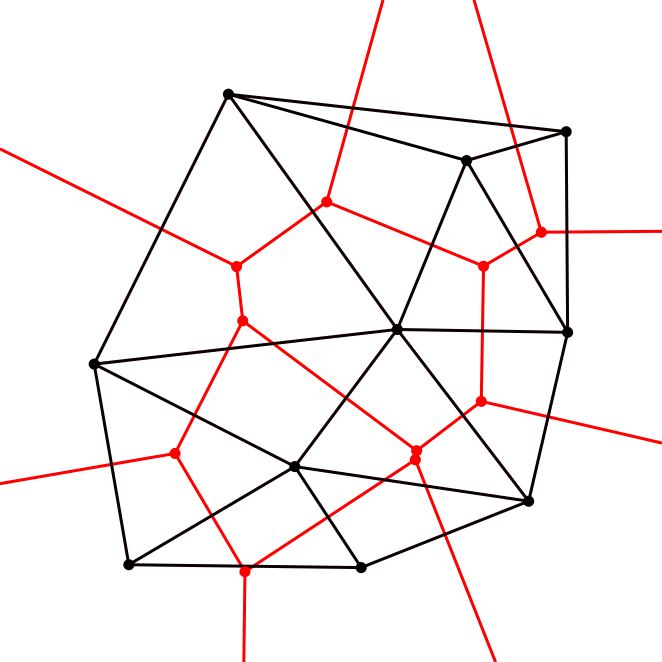
\includegraphics[width=0.6\textwidth]{kuvat/voronoi.png}
  \caption{Mustien pisteiden Delaunayn kolmiointi (mustat viivat) ja sitä vastaava Voronoin tesselaatio punaisella. Punaiset pisteet ovat Delaunayn kolmioinnissa käytettyjen ympyröiden keskipisteitä. (Kuva: Wikimedia Commons -käyttäjä \textit{Hferee}, CC BY-SA 3.0)}
  \label{voronoi}
\end{figure}

Menetelmä on yleistettävissä myös korkeampiin ulottuvuuksiin, jolloin esimerkiksi kolmiulotteisessa tapauksessa syntyy ympyröiden sisällä olevien kolmioiden sijaan pallojen sisällä olevia tetraedrejä. \cite{maur2002delaunay}

\subsection{Algoritmit}
Delaunayn kolmioinnin luomiseen on kehitetty useita erilaisia algoritmeja. Ne voidaan kuitenkin jakaa muutamaan peruskategoriaan:\cite{dewall}
\begin{itemize}
	\item \textit{Paikallinen parantaminen}, jossa aluksi luodaan mielivaltainen kolmiointi ja erilaisilla paikallisilla muunnoksilla muutetaan kolmiointi Delaunayn kolmioinniksi.
	\item \textit{Vaiheittainen lisääminen}, jossa kolmiointi rakennetaan lisäämällä kolmiointiin kolmioita yksittäin niin, että uudet kolmiot täyttävät aina kolmioinnille asetetut ehdot
	\item \textit{Vaiheittainen rakentaminen}, jossa lisätään kolmiointiin pisteet yksi kerrallaan, ja kolmio, joka sisältää lisätyn pisteen, jaetaan uusiin kolmioihin siten, että kaikki toteuttavat kolmioinnille asetetut ehdot. 
	\item \textit{Korkeampaan ulottuvuuteen upottaminen,} jossa pisteet siirretään korkeampaan ulottuvuuteen, jossa lasektaan pisteille konveksi kuori, jonka projektiosta alkuperäiseen ulottuvuuteen saadaan Delaunayn kolmiointi 
	\item \textit{Hajota ja hallitse} -algoritmit, joissa pistejoukko jaetaan rekursiivisesti pienempiin pistejoukkoihin ja nämä pistejoukot kolmioidaan. Tämän jälkeen yhdistämisvaiheessa nämä pienten alueiden kolmioinnit yhdistetään vaiheittain siten, että lopullinen kolmiointi täyttää Delaunayn kolmioinnin ehdot.
\end{itemize}

Kahdessa ulottuvuudessa monet näistä ovat yksinkertaisia, mutta kolmessa ulottuvuudessa monen algoritmin toteuttaminen muodostuu huomattavasti vaikeammaksi. Esimerkiksi neljän pisteen välille piirrettyjä kolmioita, jotka voivat toteuttaa Delaunay-kolmioinnin ehdot, on vain kaksi erilaista kun taas neljän pisteen välille voidaan kolmessa ulottuvuudessa piirtää viisi erilaista tetraedrikonfiguraatiota, jolloin ns. \textit{edge-flipping} -algoritmien toteuttaminen on huomattavasti haastavampaa. \cite{maur2002delaunay}

\subsubsection{Quickhull}\label{quickhull}
Mikäli kolmioitava kappale on konveksi ja halutaan kolmioida ainoastaan kappaleen pinta, voidaan hyödyntää suoraan jotakin konveksin kuoren etsimiseen käytettävää algoritmia\cite{maur2002delaunay}. Esimerkiksi ellipsoidin muotoisen asteroidin pinnan muotojen mallintamiseen riittää pinnan kolmiointi ilman pisteiden tetraedrointia ja ellipsoidi on konveksi kappale, joten konveksin kuoren etsimiseen käytettävät algoritmit ovat suoraan sovellettavissa tähän ongelmaan, sillä pistejoukon kovenksi kuori on tällöin suoraan pistejoukon Delaunayn kolmiointi.

Eräs nopea ja periaatteeltaan yksinkertainen myös suurille pistejoukoille sopiva konveksin kuoren etsintäalgoritmi on quickhull. Algoritmin suorittaminen aloitetaan valitsemalla pistejoukosta ensimmäinen tetraedri. Tätä varten pistejoukosta ensin minimi- ja maksimipisteet kaikkien koordinaattiakselian suunnassa (6 kpl) ja valitaan näistä ensin kaksi kauimpana toisistaan sijaitsevaa pistettä. Seuraavaksi etsitään jäljelle jääneistä neljästä pisteestä se, jonka kohtisuora etäisyys näiden pisteiden virittämästä suorasta on suurin, jolloin saadaan ensimmäisen tetraedrin pohja. Viimeisenä valitaan piste, jonka etäisyys tästä kolmiosta on suurin, jolloin on saatu luotua ensimmäinen tetraedri. \cite{quickhull}

Algoritmin suorituksen kannalta on tärkeää, että jokainen pistejoukon piste, joka ei ole syntyneen kuoren sisällä (konveksin kappaleen tapauksessa tälläisiä pisteitä ei löydy, joten nämä eivät ole tämän työn kannalta relevantteja) tai jo osana jotakin kolmiota, kuuluu jostakin olemassaolevasta kolmiosta näkyviin pisteisiin. Tästä syystä käydään alussa kukin piste läpi, ja käydään kutakin pistettä kohden läpi tahkoja, kunnes löytyy tahko, josta katsottuna kyseinen piste on horisontin yläpuolella. Kun tällainen tahko löytyy, lisätään piste tahkosta näkyvillä olevien pisteiden listaan. Todellisuudessa moni piste näkyy useista tahkoista, mutta nekin merkitään vain yhden tahkon listaan.\cite{quickhull}

Pisteen näkyvyys tahkolta voidaan tarkastaa yksinkertaisesti tutkimalla, onko piste eri puolella tahkon määräämää tasoa kuin jokin jo luodun monitahokkaan sisällä oleva piste. Omassa toteutuksessani tämä toteutetaan määrittämällä ensin kolmion määräämän tason yhtälö muodossa $ax+by+cz+d=0$, minkä jälkeen voidaan kahden pisteen koordinaatit sijoittaa yhtälön vasemmalle puolelle. Mikäli näin saadut luvut ovat samanmerkkiset, ovat pisteet samalla puolella tasoa. Merkki on yksinkertaista määrittää ottamalla lukujen tulo ja tarkastelemalla sen etumerkkiä.

Kun kaikille pisteille on löydetty tahko, josta ne näkyvät, työnnetään kaikki neljä luotua tahkoa käsiteltävien tahkojen pinoon. Tämän jälkeen aloitetaan varsinainen iteraatiovaihe, jossa monitahokasta laajennetaan, kunnes se kattaa kaikki pistejoukon pisteet.\cite{quickhull}

Iteraatiovaiheessa poimitaan pinosta päällimmäinen tahko, joka on tämän iteraation käsiteltävä. Kun käsiteltävien tahkojen pino on tyhjä, on kolmiointi valmis. Mikäli tällä tahkolla ei ole yhtään näkyvää pistettä siirrytään seuraavaan iteraatioon, muussa tapauksessa valitaan tahkon näkyvistä pisteistä kaukaisin. Tämän jälkeen etsitään edellä esitettyä näkyvyydentarkastusmenetelmää käyttäen käsiteltävän kolmion naapureista (tahkoista, jotka jakavat vähintään yhden pisteen käsiteltävän tahkon kanssa) sellaiset, joista kaukaisin piste on näkyvissä. Näitä pisteestä näkyviä tahkoja ympäröi horisontti, jonka pisteet yhdistämällä kaukaisimpaan pisteeseen, saadaan korvattua käsiteltävä ja näkyvät kolmiot uusilla, jolloin monitahokas kasvaa jonkin verran. Korvatuista kolmioista näkyvissä olevat pisteet jaetaan uusille kolmioille ja uudet kolmiot lisätään käsiteltävien kolmioiden pinoon. Korvatut kolmiot poistetaan käsiteltävien kolmioiden pinosta.\cite{quickhull}

Kuvassa \ref{quickhull-iteraatio} on nähtävillä yhden iteraation kulku Quickhull-algoritmissa. Kuvassa vasemmalla ylhäällä alkutila, jossa monitahokasta ympäröi vaaleanharmailla ympyröillä merkitty pistejoukko. Oikealla ylhäällä nähtävillä tummanpunaisella nyt käsittelyvuorossa oleva tahko. Tämän tahkon näkyvien pisteiden listassa on vain yksi piste (kirkkaanpunainen ympyrä), vaikka tahkosta todellisuudessa näkyy useita pisteitä. Ne kuuluvat kuitenkin jonkin muun tahkon näkyviin pisteisiin. Vasemmalla alhaalla on tästä pisteestä nähtävissä olevat käsiteltävän tahkon naapuritahkot merkitty punaisella ja niitä ympyröivä horisontti syaanilla. Oikealla alhaalla horisontti on yhdistetty käsiteltävään pisteeseen, jolloin syntyneet uudet kolmiot on piirretty vaaleanharmaalla. Vanhat kolmiot poistetaan, jolloin päästään kuvassa \ref{iteraatio-lopputila} esitettyyn tilaan, joka toimii seuraavan iteraation alkutilana.

\begin{figure}
  \centering
  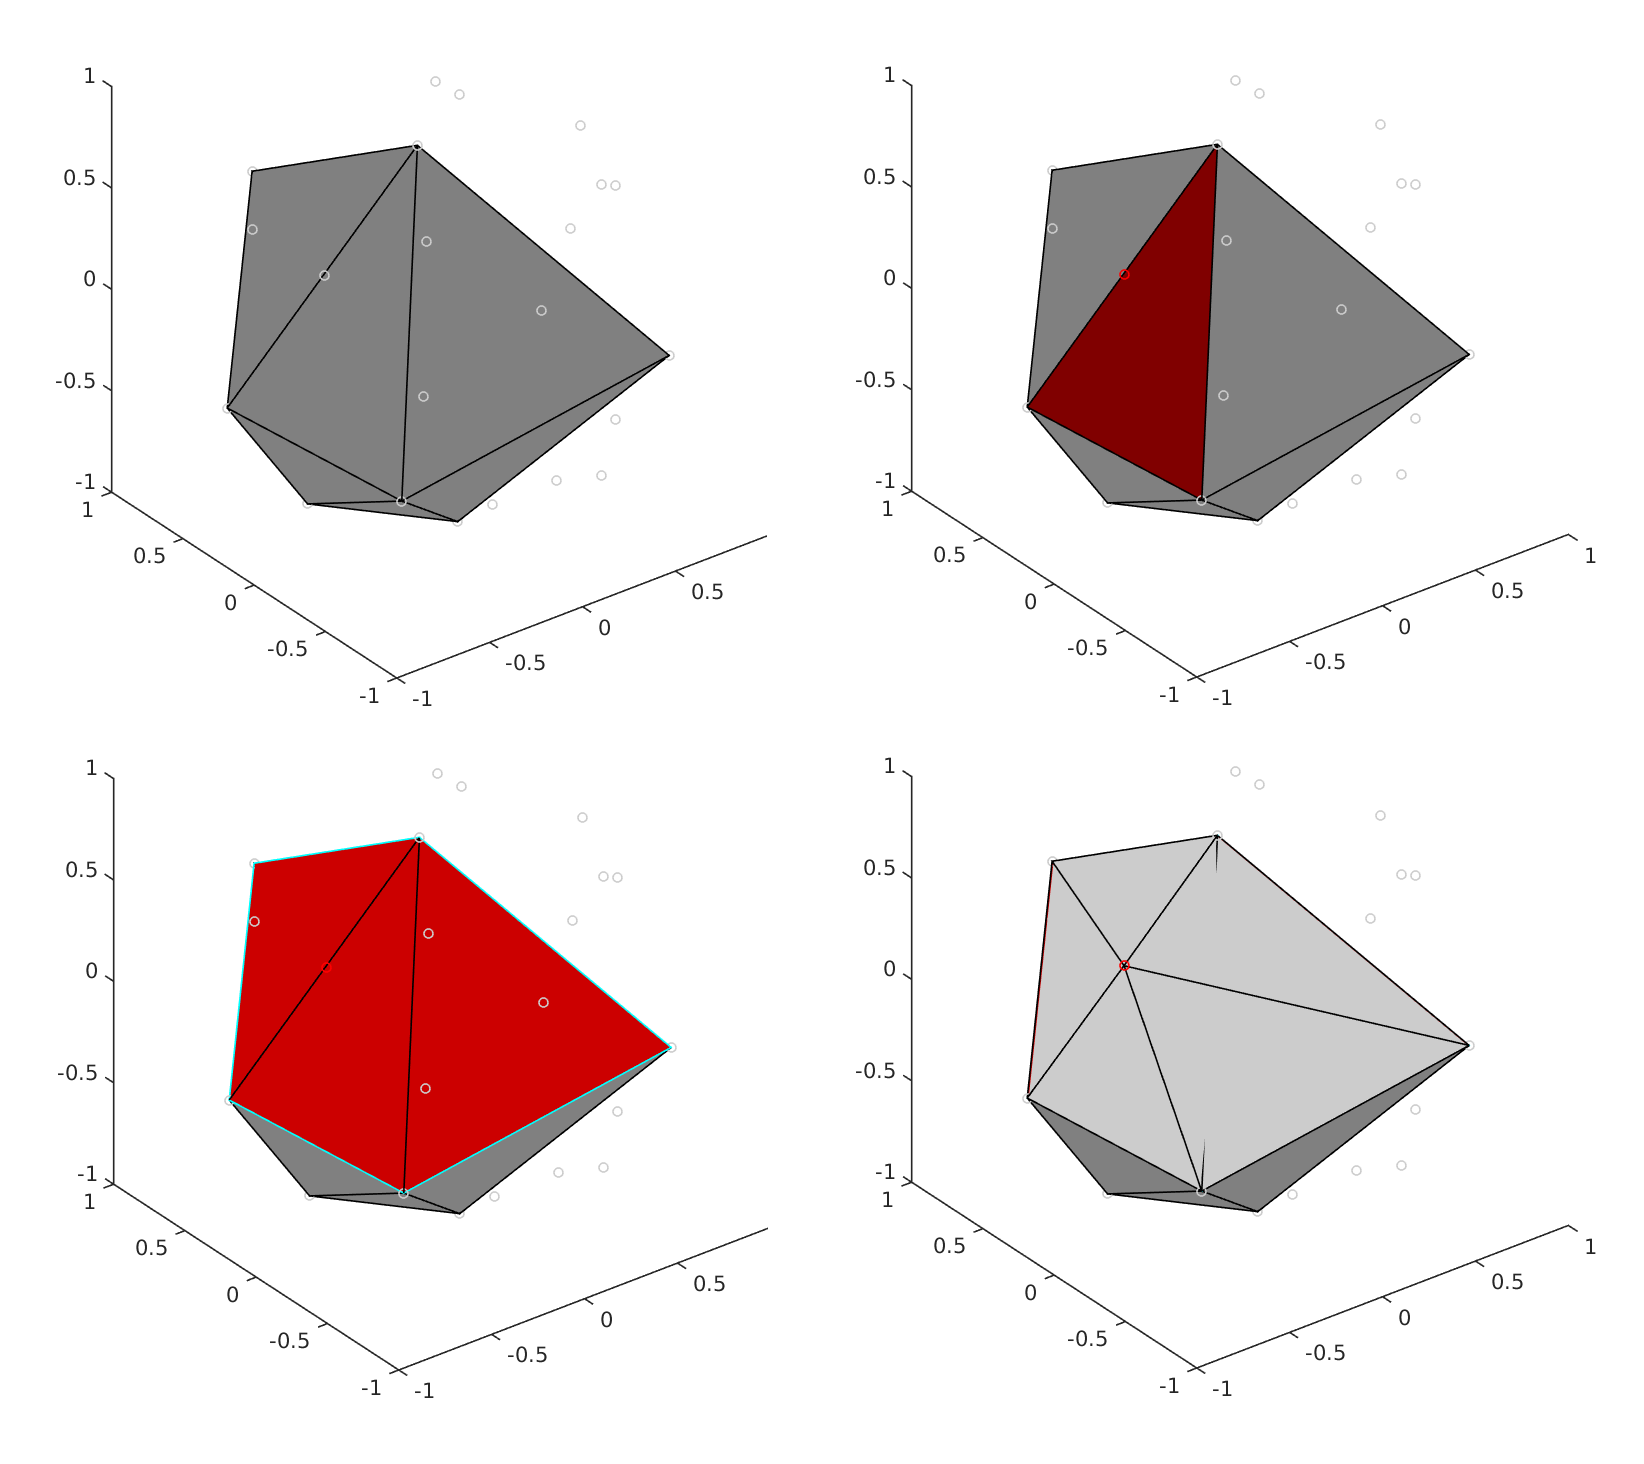
\includegraphics[width=\textwidth]{kuvat/quickhull-iteraatio.png}
  \caption{Yksi Quickhull-algoritmin iteraatio.}
  \label{quickhull-iteraatio}
\end{figure}

\begin{figure}
  \centering
  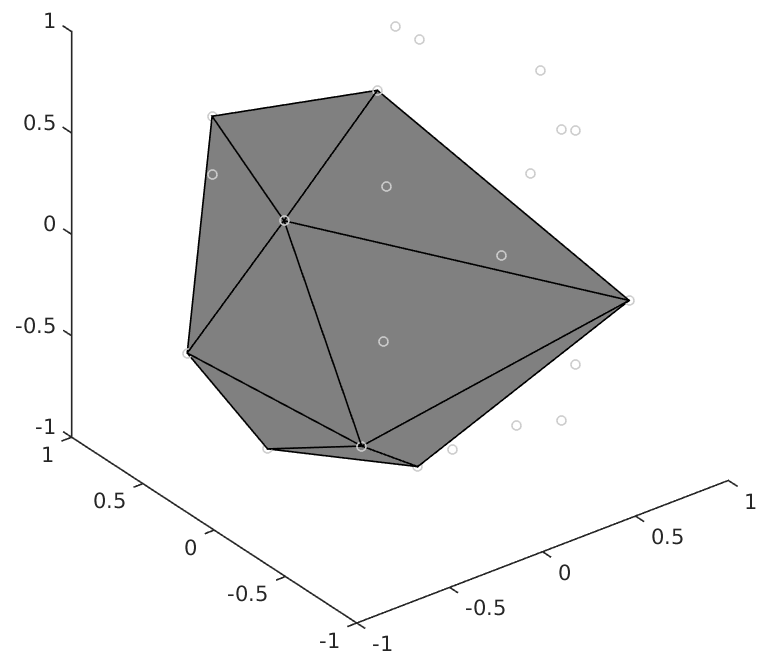
\includegraphics[width=0.8\textwidth]{kuvat/iteraatio-lopputila.png}
  \caption{Edellä esitetyn iteraation lopputila.}
  \label{iteraatio-lopputila}
\end{figure}

\section{Pisteiden generointi ellipsoidin pinnalle}
Jotkin ongelmat vaativat tutkittavan kappaleen pinnan mallintamista pistejoukkona. Tämä on helppo ensiaskel esimerkiksi kappaleen muodon kolmioinnissa. Tässä työssä keskitytään generointimenetelmiin, joita voidaan hyödyntää ellipsoidien mallinnuksessa.

Pisteiden generointiin käytettävät menetelmät voidaan jakaa karkeasti kahteen luokkaan: systemaattisiin ja satunnaisiin menetelmiin. Kummassakin pyritään yleensä luomaan mahdollisimman tasainen jakauma kappaleen pinnalle. Seuraavissa aliluvuissa esitellään yksi systemaattinen ja yksi satunnainen menetelmä.

\subsection{Pisteiden luominen kerroksittain}
Eräs yksinkertainen tapa luoda ellipsin pinnalle pistejoukko, jossa lähimpien pisteiden etäisyydet pysyvät likimain vakioina, on generoida pisteet ellipsin leveyspiirien suuntaisina kehinä. Ellipsi jaetaan $k$ kerrokseen, jolloin navalla olevaan ensimmäiseen ''kerrokseen'' tulee yksi piste, seuraavaan kerrokseen 4 ja tästä kohti päiväntasaajaa kuhunkin kerrokseen aina 4 pistettä enemmän kuin edelliseen. Päiväntasaajan jälkeen pisteiden määrä alkaa jälleen vähentyä neljällä pisteellä kerrosta kohti, kunnes vastakkaisella navalla on jälleen vain yksi piste.

Tämä on yksinkertaisinta tehdä $(\theta, \phi, r)$-koordinaatistossa, jossa $\theta$ mittaa kulmaa navalta kohti päiväntasaajaa ja $\phi$ kulmaa x-akselista positiiviseen kiertosuuntaan z-akselin ympäri. Tällä tavoin generoitaessa kunkin rivin kulmaetäisyydeksi $\theta$-suunnassa muodostuu $\pi/k$ ja kahden saman latitudin pisteen välinen etäisyys $\phi$-suunnassa on $\frac{\pi}{2(k-1)}$.

Näistä pisteistä on yksinkertaista muodostaa ellipsin pinnan kattava kolmiointi, jossa napa toimii kärkenä neljälle kolmiolle ja seuraavan rivin pisteet kussakin oktantissa yhdistävät janat kolmioiden kantoina. Seuraavalla kolmiorivillä edellisen kolmiorivin kantoja vastaa aina kärki ja kunkin oktantin reunoihin muodostuu kaksi uutta kolmiota. Näin jatketaan jälleen päiväntasaajalle asti, minkä jälkeen kolmiot alkavat jälleen vähentyä napaa lähestyttäessä. Kuva 200 kerrosta sisältävästä näin luodusta pistejoukosta on nähtävillä kuvassa \ref{murrikolmiointi}.

\begin{figure}
  \centering
  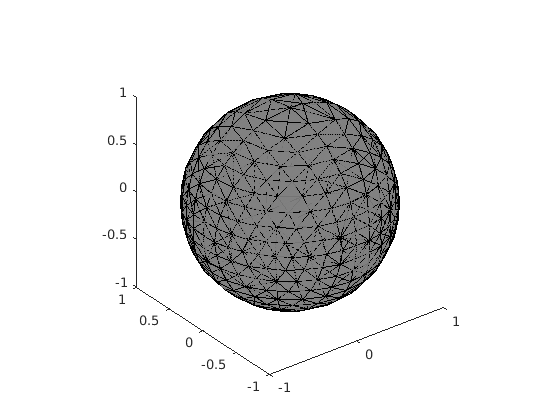
\includegraphics[width=0.6\textwidth]{../Delaunay/data/murrikolmiot/pallo.png}
  \caption{Matlabin \texttt{delanayn}-komentoa käyttäen luotu kuva kerroksittain luodusta pistejoukosta ykikköpallon pinnalla.}
  \label{murrikolmiointi}
\end{figure}

\subsection{Pisteiden arpominen}
Pisteiden generointi satunnaisesti on hyvin yksinkertainen tapa generoida vähällä vaivalla halutunkokoinen pistejoukko. Pallopinnalle generointi on erittäin yksinkertaista. Kun tiedetään haluttu pallon säde, voidaan generoida satunnaisluvut $\theta \in [0, \pi]$ ja $\phi \in [0, 2\pi]$, jolloin saadaan suoraan piste $(\theta, \phi, r)$ missä $r$ on vakio. Esimerkki näin saadusta pistejoukosta on nähtävillä kuvassa \ref{satunnaispallo}.

\begin{figure}[h]
  \centering
  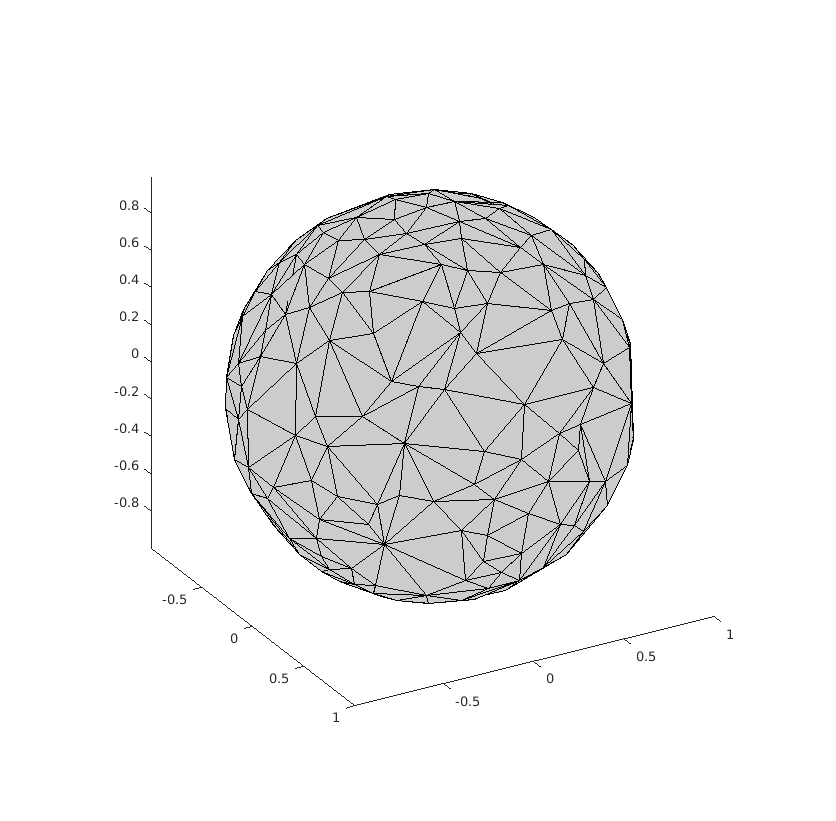
\includegraphics[width=0.8\textwidth]{../Delaunay/data/pallo250/pallo2.png}
  \caption{Yksikköpallon pinnalle satunnaisgeneroitu pistejoukkoon tehty Delaunayn kolmiointi. Pallo koostuu 250 pisteestä ja 505 niiden välille piirretystä kolmiosta.}
  \label{satunnaispallo}
\end{figure}

Ellipsoidin pinnalle generoiminen on kuitenkin monimutkaisempaa, sillä edellä kuvatulla tavalla pistejakaumasta tulee ellipsoidin eksentrisyydestä riippuen mahdollisesti hyvinkin epätasainen. Pohjimmiltaan voidaan kuitenkin käyttää samantyyppistä menetelmää kuin edellä, eli aloittaa generoimalla vastaavat kulmat $\theta$ ja $\phi$ ja määrittämällä näiden perusteella kyseisen pinnan kohdan etäisyys origosta kaavan \ref{r} perusteella, missä $a$, $b$ ja $c$ ovat ellipsin muodon määräävät parametrit ellipsin yhtälöstä (yhtälö \ref{ellipsin-yhtalo}).

\begin{equation}\label{r}
	r(\theta,\phi) = \frac{abc}{\sqrt{b^2c^2\sin^2(\phi)\cos^2(\theta)+a^2c^2\sin^2(\phi)\sin^2(\theta)+a^2b^2cos^2(\phi)}}
\end{equation}

\begin{equation}\label{ellipsin-yhtalo}
	\frac{x^2}{a^2}+\frac{y^2}{b^2}+\frac{z^2}{c^2} = 1
\end{equation}

Eräs tapa huolehtia jakauman tasaisuudesta halutulla tarkkuudella on asettaa tietty kynnysarvo kunkin pisteen ympärillä olevalle säteelle, jonka sisälle ei generoida uusia pisteitä. Tämä voidaan toteuttaa esimerkiksi jakamalla ellipsin pinta-ala halutulla pistemäärällä ja määrittämällä tätä alaa vastaavan ympyrän säde, jolloin voidaan hylätä tätä sädettä lähempänä toista pistettä olevat pisteet. Uusia pisteitä arvotaan, kunnes hyväksyttyjen pisteiden kokonaismäärä on haluttu pistemäärä.

Tätä menetelmää voidaan edelleen kehittää määrittämällä tasaisuuskerroin, jolla kerrotaan saatu ala kutakin pistettä kohden. Pienillä kertoimilla pisteet voivat olla lähempänä toisiaan, jolloin pisteitä hylätään vähemmän eli generointi on nopeampaa, mutta jakauman tasaisuus kärsii. Liian suuren kertoimen valitseminen saattaa johtaa tilanteeseen, jossa uusien kaikki ehdot täyttävien pisteiden generointi on mahdotonta. Esimerkki ellipsoidin pinnalle generoiduista pisteistä on nähtävillä kuvassa \ref{satunnaisellipsoidi}.

\begin{figure}
  \centering
  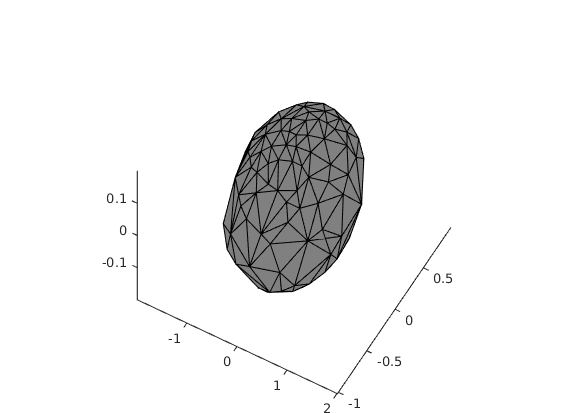
\includegraphics[width=0.8\textwidth]{../Delaunay/data/ellipsoidi150/ellipsoidi.png}
  \caption{Satunnaisgeneroidun pistejoukon Delaunayn kolmiointi ellipsin (a=1,1; b=0,8; c=0,2) pinnalla. Ellipsoidi koostuu 150 pisteestä ja 296 niiden välille piirretystä kolmiosta. Käytetty tasaisuuskerroin on 1,2.}
  \label{satunnaisellipsoidi}
\end{figure}

\section{Lommel-Seeliger -heijastuslaki}
Lommel-Seeliger -heijastuslaki käsittelee yksinkertaista heijastusta, joka tapahtuu puoliäärettömässä väliaineessa, johon valo penetroituu heikentyen absorption ja sironnan vaikutuksesta. Sirottuminen kustakin väliainekerroksesta on isotrooppista ja pintaa kohti sironnut valo heikkenee edelleen matkalla pintaan. \cite{lommel}

Tällöin heijastuskertoimeksi saadaan
\begin{equation}\label{lommel-seeliger}
	R_{Lommel-Seeliger} = \frac{1}{4}\widetilde{\omega}P_{11}(\alpha)\frac{1}{\cos(\epsilon)+\cos(\iota)},
\end{equation}
missä $\epsilon$ on havaitsijan suunnan ja heijastavan pinnan normaalin välinen kulma ja $\iota$ on valonlähteen suunnan ja heijastavan pinnan normaalin välinen kulma. \cite{tenttimatsku, lommel}.

\section{Asteroidin muodon kolmiointi}
Käytin asteroidin muodon kolmiointiin edellä esitettyä Quickhull-algoritmia. Toteutin pisteiden generointiin sekä mahdollisuudet generoida pisteet kerroksittain antamalla kerroksien määrä että mahdollisuuden generoida pisteet satunnaisesti antamalla pisteiden kokonaismäärä ja tasaisuuskerroin. Kummassakin tapauksessa annetaan lisäksi ellipsin muodon määräävät vakiot $a$, $b$ ja $c$.

Luvussa \ref{quickhull} esitetystä poiketen ylläpidin lisäksi listaa valmiista kolmioista. Varsinaista tapaa tietää, koska kolmiota on käsitelty viimeisen kerran ei ole, sillä vaikka kolmiolla ei ole omia näkyviä pisteitä, se saattaa olla nähtävissä jonkin naapurinsa näkyvästä pisteestä, jolloin se tullaan vielä poistamaan. Tästä syystä lisäsin kaikki uudet kolmiot luotaessa valmiiden listaan ja poistin sieltä aina iteraation lopuksi työstettävän kolmion ja valoisat kolmiot. Näin käsiteltävien kolmioiden pinon tyhjentyessä, sisältää valmiiden kolmioiden lista kaikki pinnan Delaunay-kolmiointiin kuuluvat kolmiot.

Ohjelma kokonaisuudessaan on nähtävissä ja ladattavissa Githubissa (\url{https://github.com/aajarven/aurfys/tree/master/Delaunay}). Projekti sisältää myös debuggauksessa ja visualisointien luonnissa käytettävää koodia, muun muassa tiedostojen kirjoittamiseen käytetyn IO-luokan. Animaatioita toteuttamani Quickhull-algoritmin toiminnasta on nähtävissä osoitteessa \url{https://www.cs.helsinki.fi/u/aajarven/delaunay/}.

\section{Asteroidin sisäinen rakenne}
Kun asteroidin pinta on kolmioitu, voidaan asteroidin sisärakenne kattaa tetraedreillä yksinkertaisesti käyttämällä kutakin kolmiota yhden tetraedrin pohjana ja ellipsoidin keskipistettä tetraedrin neljäntenä kärkenä. Paikkaresoluution parantamiseksi voidaan nämä tetraedrit edelleen jakaa ellipsoidin säteen suunnassa katkaistuihin kartioihin.

Yksinkertaisinta on tehdä jako siten, että kunkin katkaistun kartion korkeus on sama. Tällöin kuitenkin monitahokkaiden tilavuus vaihtelee säteen suunnassa: lähellä keskipistettä tilavuudet ovat pieniä ja lähellä pintaa hyvin suuria. Tästä syystä monissa sovelluskohteissa on hyödyllisempää suunnitella jako monitahokkaisiin siten, että niiden tilavuudet pysyvät likimain samoina.

Tällöin kunkin katkaistun kartion korkeuden laskeminen onnistuu, kun tunnetaan lausekkeet kartion tilavuudelle
\begin{equation}\label{kartiontilavuus}
	V=\frac{1}{3}Ah
\end{equation}
missä $A$ on kartion pohjan ala ja $h$ kartion korkeus.
% sekä katkaistun kartion tilavuudelle
%\begin{equation}\label{katkaistukartio}
%	 V = \frac{1}{3} h (A + \sqrt {AA'} + A')
%\end{equation}
%missä $A$ ja $A'$ ovat pohjien alat ja $h$ on pohjien välinen kohtisuora etäisyys. \cite{wiki:kartio}
%
%Lisäksi tiedetään, että eri katkaistujen kartioiden pohjat ovat yhdenmuotoisia ja niiden alat ovat verrannollisia ellipsoidin keskipisteestä mitatun etäisyyden neliöön. Kun nyt merkitään ellipsoidin sädettä tarkasteltavan tetraedrin kohdalla $R$ (oletetaan, että kolmiot ovat säteeseen verrattuna pieniä, jolloin matka kustakin pohjan pisteestä keskipisteeseen on likimain sama) ja katkaistun kartion korkeutta $h$, saadaan katkaistun kartion pohjien alojen suhteeksi
%\begin{equation*}
%	A_1=\left(\frac{R-h}{R}\right)^2A_0.
%\end{equation*}
%
%Jos kartio halutaan jakaa $n$ osaan, voidaan yhden osan tilavuus laskea yksinkertaisesti
%\begin{align}
%	V_{katkaistu} &= \frac{1}{n}V_{kokonainen}\nonumber\\
%	&= \frac{1}{n}\frac{1}{3}Ah \nonumber
%\end{align}
%
\begin{figure}
  \centering
  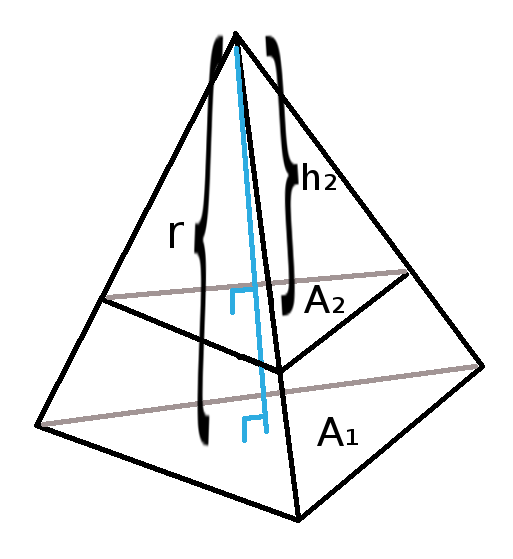
\includegraphics[width=0.6\textwidth]{kuvat/skaalaus.png}
  \caption{Katkaistujen kartioiden luomisessa käytetty notaatio.}
  \label{skaalaus}
\end{figure}

Tarkastellaan tilannetta, jossa tehdään lähinnä ellipsoidin pintaa oleva leikkaus siten, että katkaistuun kartioon jää osuus $1/n$ koko kartion tilavuudesta. Laskut on kuitenkin helpompi suorittaa, jos tarkatellaan yhden katkaisemattoman ja yhden katkaistun kartion sijaan kahta katkaistua kartiota: kuvan \ref{skaalaus} notaatiolla kartioita joiden pohjat ovat $A_1$ ja $A_2$ ja joilla on yhteinen neljäs kärki. Tällöin suuremman kartion tilavuudelle $V_1$ ja pienemmän kartion tilavuudelle $V_2$ pätee 
\begin{equation*}
	V_2 = \frac{n-1}{n}V_1
\end{equation*}
eli sijoittamalla yhtälö \ref{kartiontilavuus}
\begin{equation}\label{kartiovalivaihe}
	\frac{1}{3}A_2h_2 = \frac{n-1}{n}\frac{1}{3}A_1r.
\end{equation}

Kartioiden korkeuksien suhde määräytyy toistaiseksi tuntemattomalla tavalla kartioiden lukumäärän perusteella. Merkitään tätä suhdetta $k_2$ siten, että $r=k_2h_2$. Kartioiden pohjat ovat yhdenmuotoisia ja niiden pinta-ala on verrannollinen keskipisteestä mitatun etäisyyden neliöön, siis $A_2=k_2^2A_1$. Sijoitetaan nämä yhtälöön \ref{kartiovalivaihe}, jolloin saadaan:
\begin{equation}\label{kartiovalivaihe}
	\frac{1}{3}A_1k_2^2rk_2 = \frac{n-1}{n}\frac{1}{3}A_1r.
\end{equation}
Jaetaan puolittain pois molemmilla puolilla esiintyvät termit:
\begin{equation}\label{kartiovalivaihe}
	k_2^3 = \frac{n-1}{n}
\end{equation}

Näin ollen ensimmäisen katkaistun kartio, jossa on osuus $1/n$ koko kartion tilavuudesta, pienempi pohja on etäisyydellä $\sqrt[3]{\frac{n-1}{n}}r$ ellipsoidin keskipisteestä. Seuraavan katkaistun kartion suurempana pohjana toimii edellisen kartion pienempi pohja ja pienemmän pohjan etäisyys keskipisteestä voidaan laskea vastaavalla menettelyllä kuin äsken. Seuraavan jaon tapauksessa kuitenkin ''kokonaisen'' kartion tilavuus on $V_2=\frac{n-1}{n}V_1$ ja siitä halutaan leikata pienempään kartioon osuus $\frac{n-2}{n-1}$, jolloin pohjien $A-2$ ja $A_3$ väliin jäävään katkaistuun kartioon jää jälleen tilavuus $\frac{1}{n}V_1$. Päättelyketju voidaan muilta osin toistaa jälleen samanlaisena. 

Yleiselle $m$. kartiolle (pohjan ala $A_m$, korkeus $h_m=rk_m$) pätee
\begin{equation*}
	\frac{V_m}{V_1} = \frac{n-(m-1)}{n} = \frac{n-m+1}{n}.
\end{equation*}
Sijoittamalla tähän kartioin tilavuuden lausekkeet, saadaan
\begin{equation*}
	\frac{1}{3}A_mh_m = \frac{n-m+1}{n}\frac{1}{3}A_1r.
\end{equation*}
Sijoitetaan tähän $h_m=k_mr$ ja $A_m=A_1k_m^2$ ja supistetaan pois molemmilla puolilla esiintyvät termit:
\begin{equation} \label{k-yhtalo}
	k_m^3= \frac{n-m+1}{n}.
\end{equation}

Yhtälön \ref{k-yhtalo} perusteella kartio saadaan jaettua $n$ tilavuudeltaan yhtä suureen osaan, kun sitä leikataan pohjan kanssa yhdensuuntaisilla tasoilla siten, että leikkaavien tasojen etäisyys $h_m$ kartion kärjestä on
\begin{equation}
	h_m=\sqrt[3]{\frac{n-m+1}{n}}r,
\end{equation}
missä $m$ on kokonaisluku väliltä $[1, n]$.

%Asetetaan yhtälössä \ref{katkaistukartio} esitetyn katkaistun kartion tilavuus yhtäsuureksi tämän lausekkeen kanssa, jolloin tiedetään
%\begin{align}\label{katkaistunkorkeus}
%	\frac{1}{3} h (A + \sqrt {AA'} + A') &= \frac{1}{n}\frac{1}{3}Ah &\bigg\vert~ A'=\left(\frac{R-h}{R}\right)^2A \nonumber\\
%	h \left(A + \sqrt {A^2\left(\frac{R-h}{R}\right)^2} + \left(\frac{R-h}{R}\right)^2A\right) &= \frac{1}{n}Ah & \nonumber\\
%	A\left(1 + \frac{R-h}{R} + \left(\frac{R-h}{R}\right)^2\right) &= \frac{1}{n}A &\nonumber\\
%	1 + \frac{R-h}{R} + \left(\frac{R-h}{R}\right)^2 &= \frac{1}{n} &\nonumber\\
%	1 + 1-\frac{h}{R} + \left(1-\frac{h}{R}\right)^2 &= \frac{1}{n} &\nonumber\\
%	1 + 1-\frac{h}{R} + 1-2\frac{h}{R}+\left(\frac{h}{R}\right)^2 &= \frac{1}{n} &\nonumber\\
%	3 - 3\frac{h}{R} +\left(\frac{h}{R}\right)^2 &= \frac{1}{n} &
%\end{align}

%Yhtälö \ref{katkaistunkorkeus} on yksinkertainen toisen asteen yhtälö, josta voidaan helposti ratkaista h. Seuraavan katkaistun kartion korkeus saadaan käyttämänä suuremman pohjan alana $A$ ulomman kartion osan pienempää pohjaa $A'$, kokonaisen kartion korkeutena matkaa $R-h$ ja tämä pienempi kartio jaetaan nyt $n-1$ osaan. Näin voidaan käyttää samaa lähestymistapaa myös seuraavaan kerrokseen.
	
\section{Asteroidin integroitu kirkkaus}
Kolmioidun asteroidin integroitu kirkkaus saadaan yksinkertaisesti laskemalla yhteen havaitsijan havaitsemat kirkkaudet eri kolmioista. Toteutin tämän siten, että aluksi lasketaan kolmion normaali, joka suuntautuu poispäin origosta. Kolmion kärkipisteiden perusteella mahdollisia normaaleja on kaksi, ja näistä valitaan se, jonka pistetulo origon (origo on väistämättä origokeskisen ellipsoidin sisällä) ja jonkin kolmion kärkipisteen välisen paikkavektorin kanssa on yli nolla eli vektorien välinen kulma ei ole yli 90$^\circ$. Tämän normaalivektorin ja Auringon sekä havaitsijan paikkavektorien (asteroidikeskeisessä koordinaatistossa) välisistä kulmista saadaan kulmat $\epsilon$ ja $\iota$. Mikäli kumpi tahansa kulmista $\epsilon$ ja $\iota$ on välin $[-\pi/2, \pi/2]$ ulkopuolella, voidaan kirkkaus asettaa suoraan nollaan, sillä kolmio ei joko ole havaittavissa tai se ei ole valaistu. Muussa tapauksessa näistä voidaan edelleen laskea yhtälön \ref{lommel-seeliger} mukaisesti heijastuskerroin.

Kirkkauden laskemisen yksinkertaisuudesta huolimatta jäi toteutukseeni bugi, jonka takia sen antamat kirkkauksien arvot eivät ole fysikaalisia, eikä minulla valitettavasti ole aikaa etsiä enää tätä bugia. Rajoitutaan tästä syystä tarkastelemaan teoreettista mallia kirkkaudelle.

Analyyttisen mallin perusteella Lommel-Seeliger -heijastuslain mukaan valoa heijastavan asteroidin kirkkaus määräytyy seuraavasti:
\begin{align}
	L_{Lommel-Seeliger} &= \frac{1}{8} \pi F_0 \widetilde{\omega} P(\alpha)abc\frac{S_{\astrosun} S_{\oplus}}{S} \{ \cos(\lambda'-\alpha') + \cos\lambda' + \sin \lambda' \sin(\lambda'-\alpha') \times\nonumber\\
	&\times\ln\left[\cot(\frac{1}{2}\lambda')\cot\frac{1}{2}(\alpha'-\lambda')\right] \},
\end{align}
missä $\alpha$ on havaitsijan ja valonlähteen välinen kulma asteroidilta katsottuna ja muut vakiot on määritelty seuraavasti, kun $\vec{e}_{\astrosun}$ on valonlähteen suunnan kertova yksikkövektori ja $\vec{e}_{\oplus}$ havaitsijan suunnan kertova yksikkövektori: 
\begin{align*}
	S_{\astrosun} &= \sqrt{e_{\astrosun}^TCe_{\oplus}} \\
	S_{\oplus} &= \sqrt{e_{\oplus}^TCe_{\astrosun}} \\
	\cos(\alpha') &= \frac{e_{\astrosun}^TCe_{\oplus}}{S_{\astrosun}S_{\oplus}} \\
	\sin(\alpha') &= \sqrt{1-\cos^2(\alpha')} \\
	S &= \sqrt{S_{\astrosun}^2+S_{\oplus}^2+2S_{\astrosun}S_{\oplus}\cos(\alpha')} \\
	\cos(\lambda') &= \frac{S_{\astrosun}+S_{\oplus}\cos(\alpha')}{S} \\
	\sin(\lambda') &= \frac{S_{\oplus}\sin(\alpha')}{S}.
\end{align*}
Näissä esiintycä $C$ on määrittää ellipsin muodon. Se on muutoin nollamatriisi, mutta sen diagonaalilla on alkiot $\frac{1}{a^2}$, $\frac{1}{b^2}$ ja $\frac{1}{c^2}$. \cite{murri}

%%%%% Sisältö loppuu, lähdeluettelo %%%%%
\newpage
\bibliographystyle{plain}
\bibliography{lahteet} %lähdeluettelon tiedot tiedostossa selkkarilahteet.bib. Esimerkiksi helkasta saa kirjojen tiedot valmiiksi bibtex-muodossa, kannattaa hyödyntää.
\end{document}
